\documentclass[a4paper, 12pt]{article}

\usepackage[english, russian]{babel}
\usepackage[T2A]{fontenc}
\usepackage[utf8]{inputenc}
\usepackage{mathtext}
\usepackage{amsfonts}
\usepackage{ amssymb }
\usepackage{amsmath}
\usepackage{graphics}
\usepackage{graphicx}
\usepackage{wrapfig}
\usepackage{geometry}
\usepackage{float}
\geometry{
	a4paper,
	total={170mm, 257mm},
	left=20mm,
	top=10mm}
	
\title{Лабораторная работа 3.1.3 \\ Измерение магнитного поля Земли}
\author{Абакшин Василий, Б05-207}
\date{8 ноября 2023 г.}
\usepackage{float}

\begin{document}
	\maketitle
	
	\textbf{Цель работы:} исследовать свойства постоянных неодимовых магнитов; измерить с их помощью горизонтальную и вертикальную составляющие индукции магнитного поля Земли и магнитное наклонение.
	
	\textbf{В работе используются:} неодимовые магниты; тонкая нить для изготовления крутильного маятника; медная проволока; электронные весы; секундомер; измеритель магнитной индукции; штангенциркуль; брусок, линейка и штатив из немагнитных материалов; набор гирь и разновесов.
	
	\section*{Краткие теоретические сведения}
	
	\subsection*{Магнитный диполь}
	Магнитный момент магнитного диполя может быть рассчитан по формуле:
	\[\mathbf{m} = I\mathbf{S} \ (\text{СИ}), \ \ \ \mathbf{m} = \frac{I\mathbf{S}}{c} \ (\text{СГСЭ})\]
	Поле точечного диполя:
	\[\textbf{B}_\text{дип} = \frac{\mu_0}{4\pi}\left(\frac{3(\mathbf{m} \cdot \textbf{r})\textbf{r}}{r^5} - \frac{\textbf{m}}{r^3}\right) \ (\text{СИ}), \ \ \ \textbf{B}_\text{дип} = \frac{3(\mathbf{m} \cdot \textbf{r})\textbf{r}}{r^5} - \frac{\textbf{m}}{r^3} \ (\text{СГСЭ}) \]
	Во внешнем магнитном поле с индукцией $\textbf{B}$ на точеный магнитный диполь $\mathbf{m}$ действует механический момент сил $$\textbf{M}=[\mathbf{m}, \textbf{B}]$$
	При этом потенциальная энергия которой обладает диполь с постоянным $\mathbf{m}$, равна 
	$$W = -(\mathbf{m} \cdot \textbf{B})$$
	Когда диполь ориентирован вдоль внешнего поля, он находится в состоянии равновесия. При этом если $\mathbf{m} \uparrow \uparrow B$, то равновесие устойчивое (минимум энергии), если $\mathbf{m} \uparrow \downarrow B$, то равновесие неустойчивое (максимум энергии).
	В неоднородном поле на магнитный диполь действует сила: 
	
	\[\textbf{F} = (\mathbf{m} \cdot \nabla)\textbf{B},\]
	 В частности, проекция на ось $x$ имеет вид
	\begin{equation*}
		F_x = \mathbf{m}_x\frac{\partial B_x}{\partial x} + \mathbf{m}_y\frac{\partial B_x}{\partial y} + \mathbf{m}_z\frac{\partial B_x}{\partial z}.
	\end{equation*}
	То есть магнитный диполь в неоднородном поле ориентируется вдоль силовых линий и втягивается в область сильного поля.\\
	Сила, с которой взаимодействуют 2 магнита, оси которых сонаправлены:
	\begin{equation}
		\label{6}
		F_{12}= \mathbf{m}_1 \frac{\partial{B_2}}{\partial{r}} = \mathbf{m}_1\frac{\partial{(2\mathbf{m}_2/r^3)}}{\partial{r}} = -\frac{6 \mathbf{m}_1\mathbf{m}_2}{r^4} \;(\text{ед}.\; \text{СГС}).
	\end{equation}
	(при использовании системы СИ нужно домножить на $\mu_0 / 4\pi$). Здесь магниты притягиваются, если их магнитные моменты сонаправлены, и отталкиваются, если направлены противоположно.
	
	
	\subsection*{Неодимовые магниты}
	
	В работе используются неодимовые магниты шарообразной формы. Магнитное поле намагниченного шара на расстояниях $r \geq R$ от центра шара совпадает с полем точечного магнитного диполя, расположенного в центре, магнитный момент $\mathbf{m}$ которого совпадает с полным моментом шара. Внутри шара магнитное поле однородно и равно
	\[\textbf{B}_{0} = \frac{\mu_0 \mathbf{m}}{2\pi R^3}\]
	
	В качестве ещё одной характеристики материала магнита используют остаточную намагниченность $\textbf{M}$. $$\mathfrak{m}= \textbf{M}V ,$$ где $\displaystyle V = \frac{4\pi}{3}R^3$ - объём магнита. Величину $\textbf{B}_r = \mu_0 \textbf{M}$ называют остаточной индукцией материала (в СГСЭ $B_r = 4\pi \mathbf{M}$).
	Из сказанного выше нетрудно видеть, что индукция $\textbf{B}_p$ \textit{на полсюсах} однородно намагниченного шара направлена по нормали к поверхности и совпадает поэтому с индукцией внутри шара $\textbf{B}_p = \textbf{B}_0$. Величина $B_p$ связана с остаточной индукцией $B_r$ соотношением \[B_p = B_o = \frac{2}{3}B_r \]
	
	
	\subsection*{Определение магнитного момента магнитных шариков}
	
	\textbf{Метод А.} Величину магнитного момента $\mathfrak{m}$ двух одинаковых шариков можно рассчитать, зная их массу $m$ и определив максимальное расстояние $r_{max}$, на котором они еще удерживают друг друга в поле тяжести. При максимальном расстоянии сила тяжести шариков $mg$ равна силе их магнитного притяжения. 
	
	\begin{wrapfigure}{r}{0.25\textwidth}
			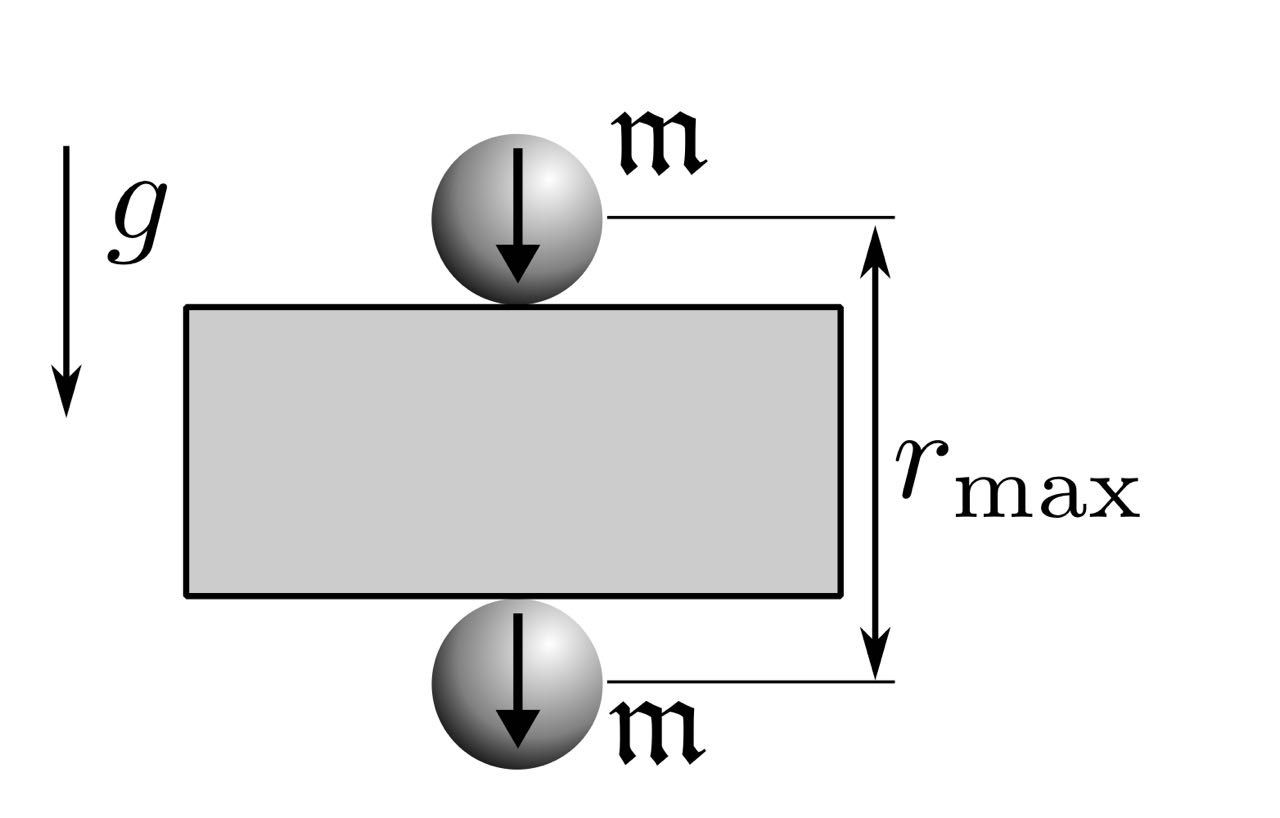
\includegraphics[width=0.4\textwidth, height = 0.2\textheight]{rmax (1)}
	\end{wrapfigure}
	
	Когда векторы двух магнитных моментов ориентированы вертикально, имеем
	
	\begin{equation*}
		\mathbf{m} = \sqrt{\frac{2\pi mgr^4_{max}}{3 \mu_0}} \ \text{(ед. СИ).}
	\end{equation*}
	
	\textbf{Метод Б.} Величину магнитного момента шариков можно определить также по силе их сцепления. Она определяется как сила, необходимая для разрыва двух сцепившихся магнитных шариков. 
	
	\begin{wrapfigure}[8]{r}{0.25\textwidth}
		\centering
		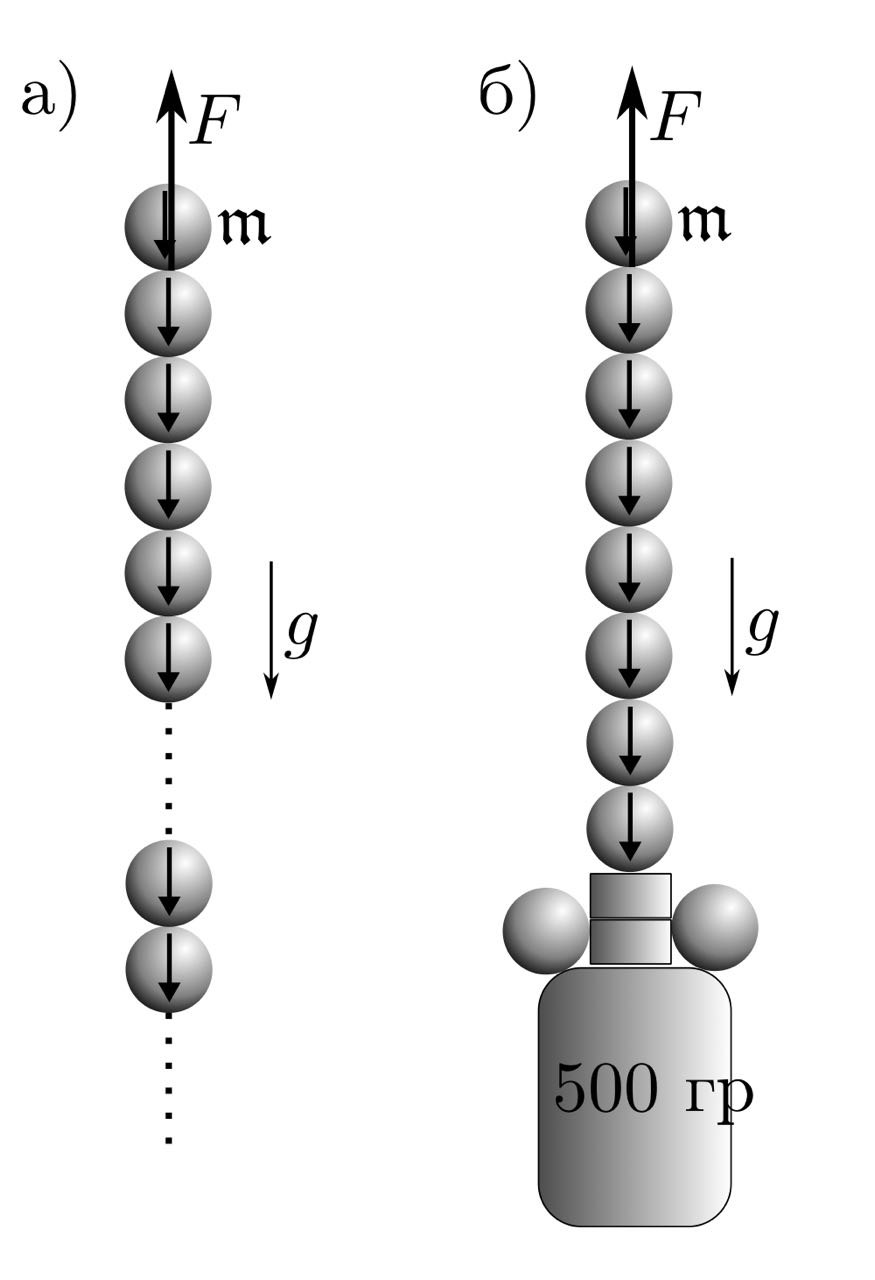
\includegraphics[width=0.3\textwidth, height = 0.25\textheight]{mmax}
		
	\end{wrapfigure}
	
	Максимальную силу сцепления можно определить по весу магнитной цепочки, которую способен удержать самый верхний магнитный шарик. Если цепь состоит из одинаковых магнитных шариков, то при определённой длине она отрывается от верхнего шарика. При этом, учитывая, что сила притяжения убывает как $F \propto 1/r^4$, где $r$ — расстояния между центрами шаров, для расчета прочности цепочки достаточно учитывать силу взаимодействия верхнего шара с 3–4 ближайшими соседями.
	
	Сила сцепления двух одинаковых шаров радиусами $R$ с магнитными моментами $\mathbf{m}$ равна 
	
	\begin{equation*}
		F_0 = \frac{3 \mu_0 \mathfrak{m}^2}{32 \pi R^4}\  \text{(ед. СИ).}    
	\end{equation*}
	
	Тогда минимальный вес цепочки, при котором она оторвётся от верхнего шарика, равен
	
	\begin{equation*}
		F = F_0\left(1 + \frac{1}{2^4} + \frac{1}{3^4} + ... \right) \approx 1,08F_0.
	\end{equation*}
	
	\vspace{2cm}
	
	\section*{Результаты измерений и обработка данных}
	В начале были проведены подготовительные измерения, данные которых приведены в таблице \ref{prep}.
	\begin{table}[H]
		\centering
		\begin{tabular}{|c|c|c|}
			\hline $d$, см & $m$, г & $B_{p1}$, мТл \\ \hline
			$0,6 \pm 0,01$   & $0,829 \pm 0,001$ &  $158 \pm 2$  \\ \hline
		\end{tabular}
		\caption{Подготовительные измерения}
		\label{prep}
	\end{table}
	\subsection*{Измерение магнитного момента шара}
	
	\textbf{Метод $\mathbf{A}$}. Предельное расстояние, на котором шарики удерживали друг друга в поле силы тяжести: $r_{max} = 1,75 \pm 0,05$ см + надо еще не забыть про расстояния от бумаги до центров шаров, то есть $r_{max}  = 2,35 \pm 0,05$ см.\\ Тогда по формуле $\mathbf{m}_1 = (6,43 \pm 0,39) \cdot 10^{-2} \ \text{Дж}/\text{Тл} \ (\varepsilon = 6 \%)$.
	
	\textbf{Метод Б}. Предельная масса груза $m_{max}=  274,33 \pm 3 $ г (погрешность весов достаточно мала, её не учитываем, но понять ровную границу, когда груз отрывается достаточно сложно). Тогда $\mathbf{m}_2 = (7,33 \pm 0,24) \cdot 10^{-2}  \ \text{Дж}/\text{Тл} \ (\varepsilon = 3,2 \%)$
	
	Оба метода не являются точными, так как многое зависит от руки экспериментатора: в первом случае он может сжать бумагу слишком сильно при измерении слоя штангенциркулем. Во втором случае можно неправильно определить максимальный вес, если двигать цепочку с ускорением. В любом случае, погрешность второго метода у нас ниже, поэтому будет использовать данные из второго способа.
	
	Рассчитаем намагниченность материала: $\mathbf{M} = \frac{\mathbf{m}}{V} = 	(64,84 \pm 3,74) \cdot 10^4 \ \frac{\text{Тл} \cdot \text{м}}{\text{Гн}} \ \ (\varepsilon = 5,77 \%)$
	Тогда остаточная индукция: 
	\[B_r = \mu_0 M = 4\pi \cdot 10^{-7} M = (0,814 \pm 0,047) \ \text{Тл} \ \ (\varepsilon = 5,77 \%) \]
	
	Можем также рассчитать индукцию на полюсе магнита: $B_p = \frac{2}{3}B_r = (0,542 \pm 0,031)$ Тл, что сильно отличается от показаний прибора. Скорее всего, прибор очень неточный, либо мы неправильно им пользовались.
	
	\subsection*{Определение горизонтальной проекции магнитного поля Земли}
 	
	Была собрана установка для измерения периода малых колебаний магнитной стрелки. Данные измерений приведены в таблице.
	
	\begin{figure}[H]
		\centering
		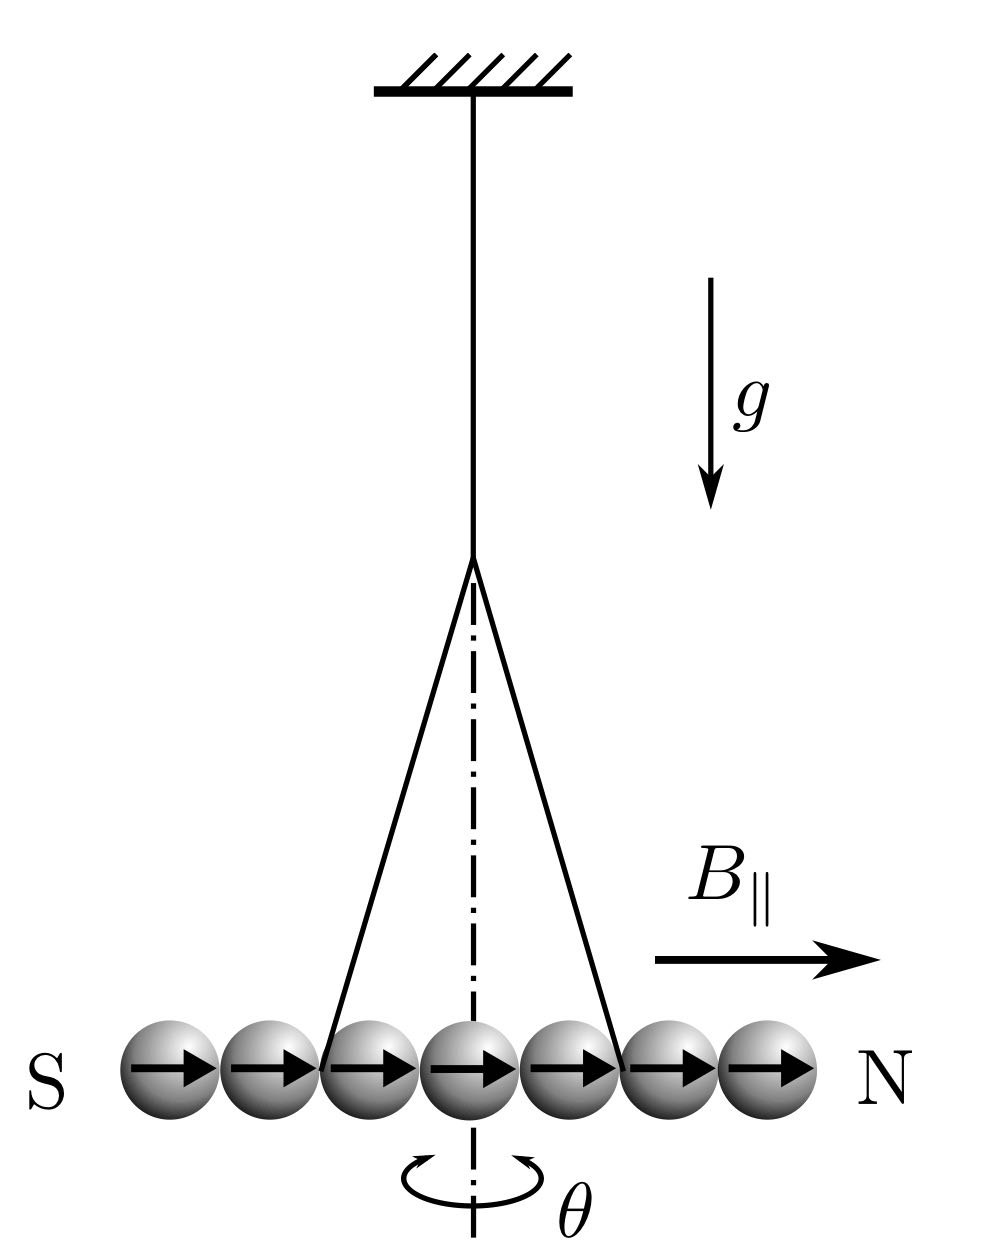
\includegraphics[scale=0.15]{horiz}
		\label{horiz}
		\caption{Крутильный маятник во внешнем магнитном поле}
	\end{figure}
	
	\begin{table}[h]
		\centering
		\begin{tabular}{|c|c|c|c|}
			\hline  $n_{\text{шар}}$ & $n_{\text{колеб}}$ & $t$, с & $T$, с \\ \hline
			5 & 5 &  9,78 & 1,96 \\ \hline
			6  & 5 &  12,63 & 2,53 \\ \hline
			7  & 5 &  11,79 & 2,36  \\ \hline
			8  & 5 &  12,91 & 2,58  \\ \hline
			9  & 3 &  9,07 & 3,02 \\ \hline
			10  & 3 &  10,63 & 3,54  \\ \hline
			11  & 3 & 14,22 & 4,74 \\ \hline
			12 & 2 & 12,41 & 6,21 \\ \hline
		\end{tabular}
		\caption{Зависимость периода колебаний от количества шариков в магнитной стрелке}
	\end{table}
	
	В график мы не включили две последние точки, они сильно выбиваются из линейной зависимости, вероятно, из-за того, что с таким количеством шариков колебания быстро затухали и мы не могли измерить достаточное их количество, чтобы минимизировать погрешность. Кроме того, в лабораторной работе предполагается, коэффициент затухания мал и тогда колебания описываются уравнением незатухающих свободных колебаний.\\
	При малых колебаниях : 
	\[J_n\theta'' + \mathbf{m}_nB_h \theta = 0, \ \ J_n = \frac{1}{3}n^3mR^2, \ \ \mathbf{m}_n = \mathbf{m} \cdot n  \]
	Отсюда находим период колебаний: 
	
	\begin{equation*}
		T(n) = 2\pi \sqrt{\frac{mR^2}{3 \mathfrak{m} B_{h}}} \cdot n, \quad \quad \frac{T(n)}{n} = k
	\end{equation*}
	
	\[B_h = \frac{4\pi^2 mR^2}{3k^2\mathbf{m}} = (2,34 \pm 0,59) \cdot 10^{-5} \ \ \text{Тл} \ \ (\varepsilon = 25\%)\]
	
	\begin{figure}[h!]
		\centering
		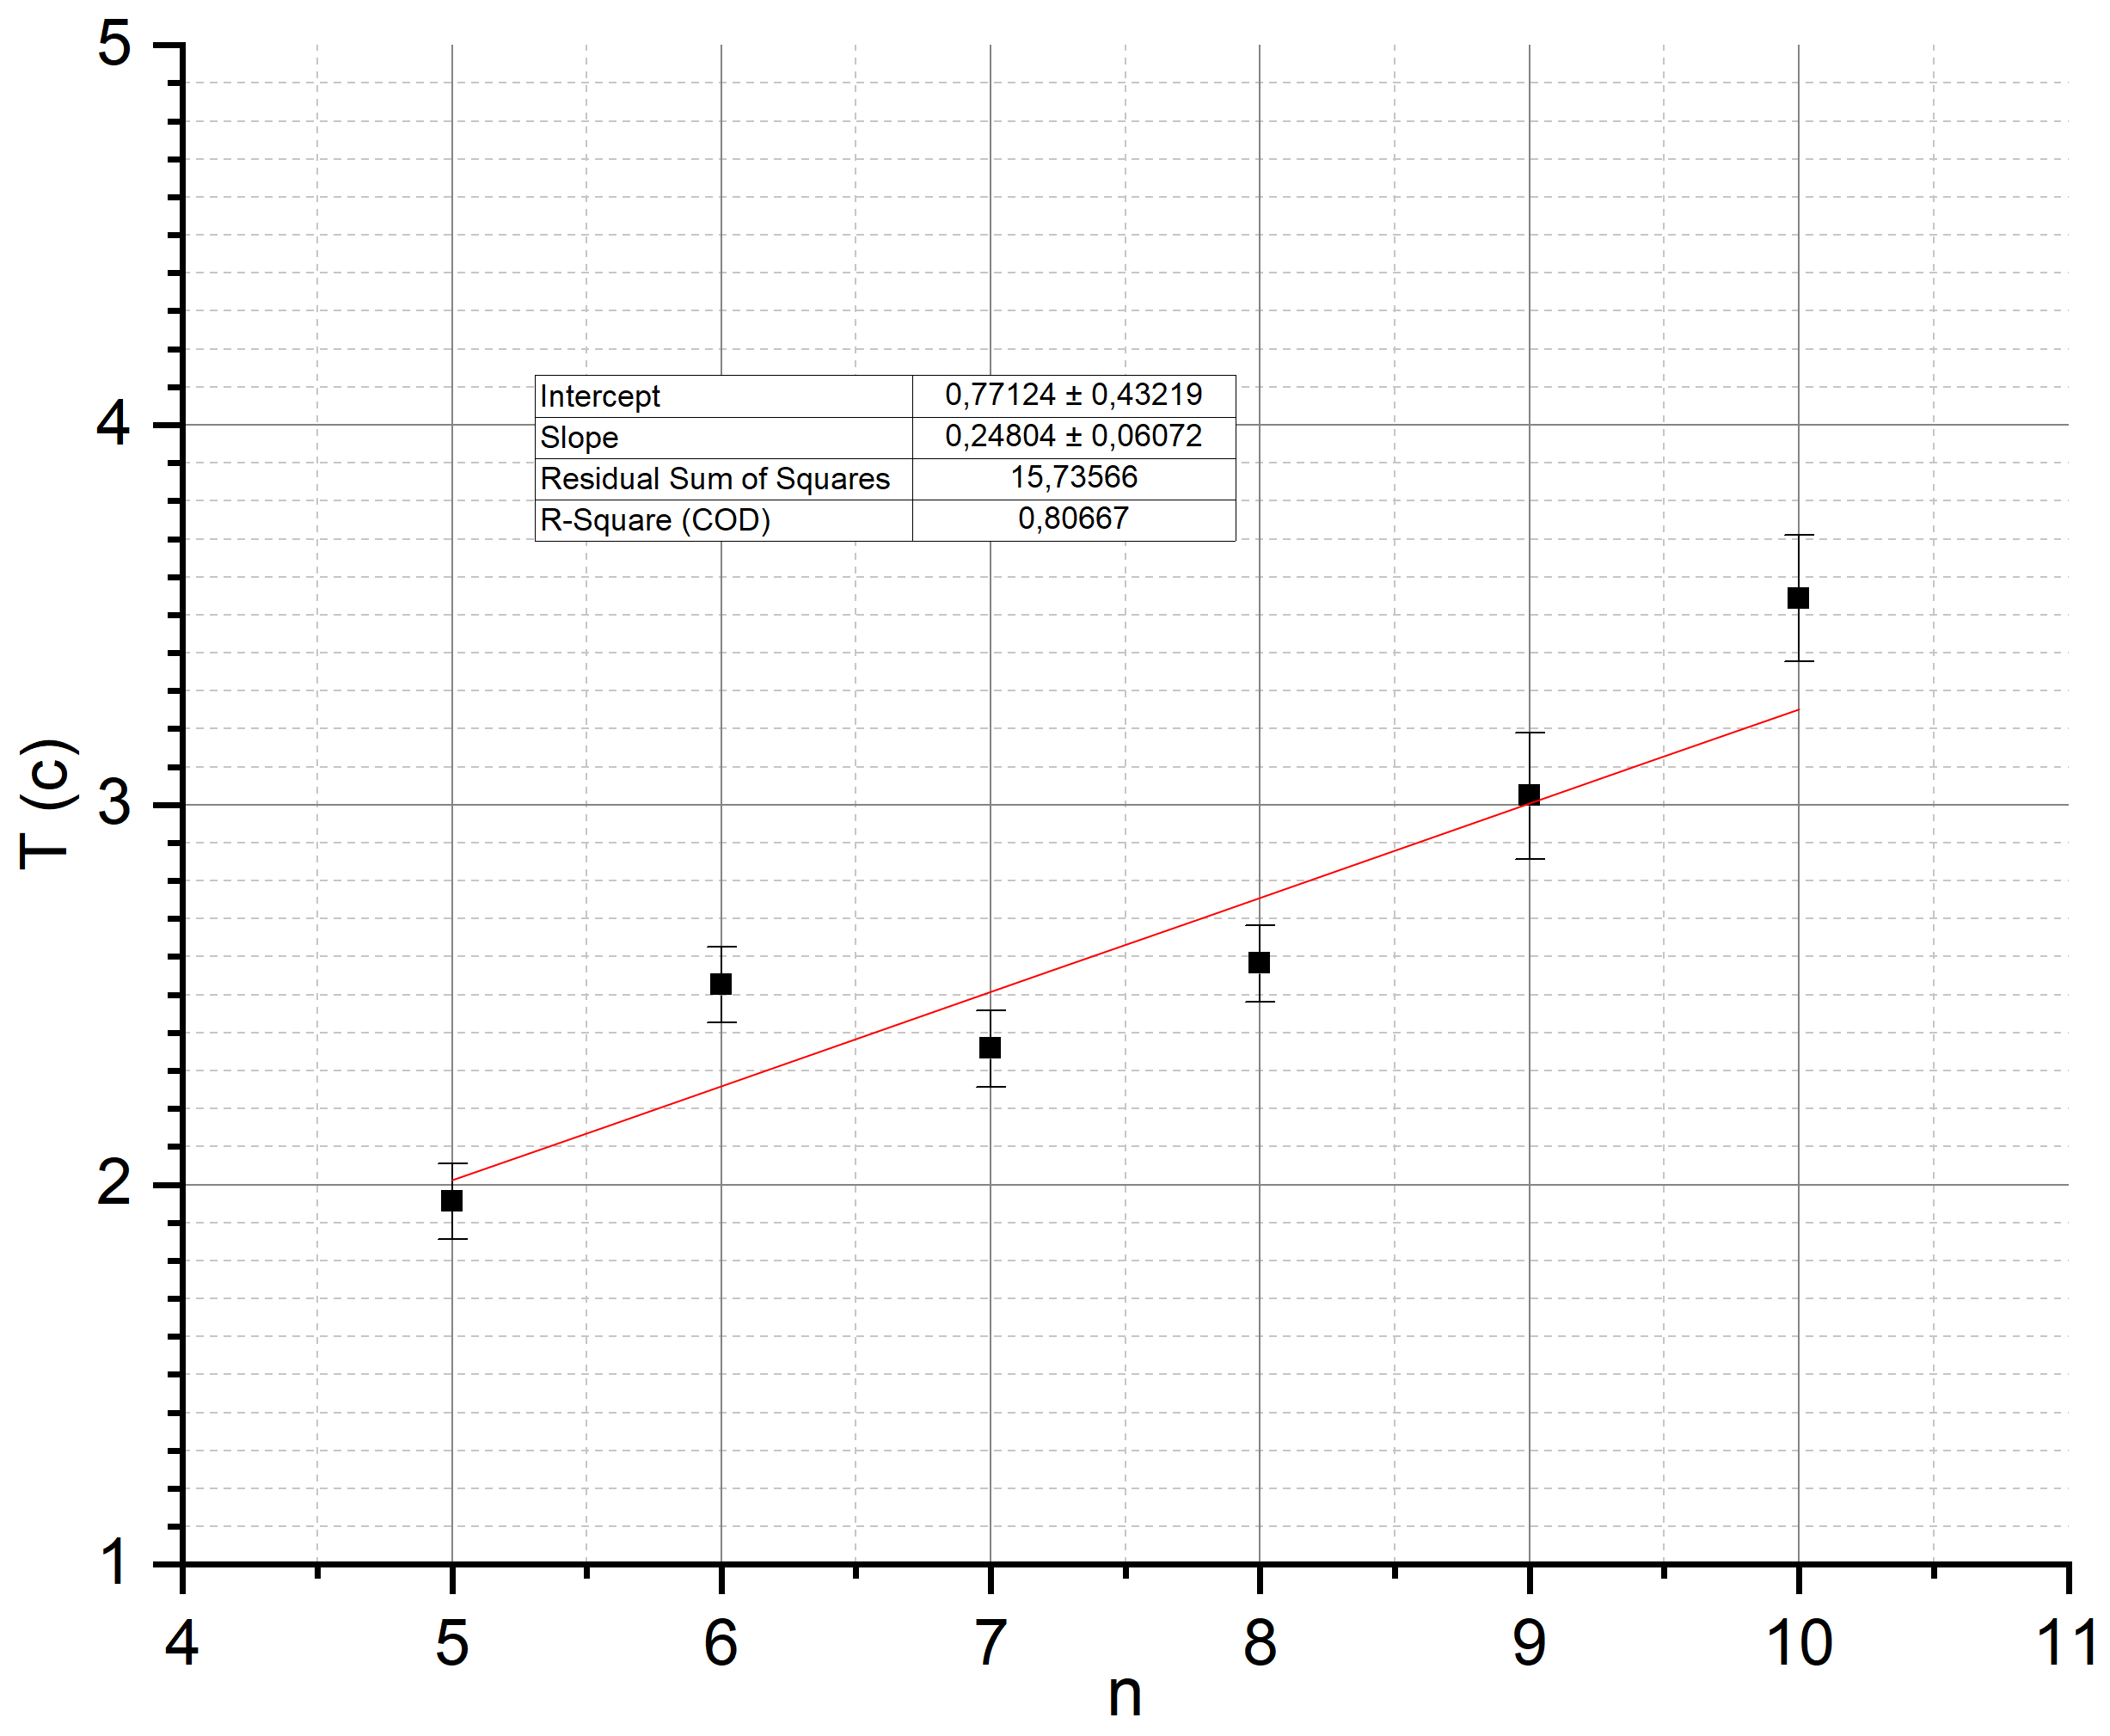
\includegraphics[width = \textwidth]{T(n)}
		\caption{\centering{График зависимости периода колебаний от количества шариков в магнитной стрелке}}
	\end{figure}
	
	\subsection*{Определение вертикальной проекции магнитного поля Земли}
	Подвешиваем четное число шариков за центр и пытаемся уравновесить момент сил магнитного поля с помощью дополнительных грузиков в виде проволок. Были получены следующие данные:
	
	\begin{figure}[H]
		\centering
		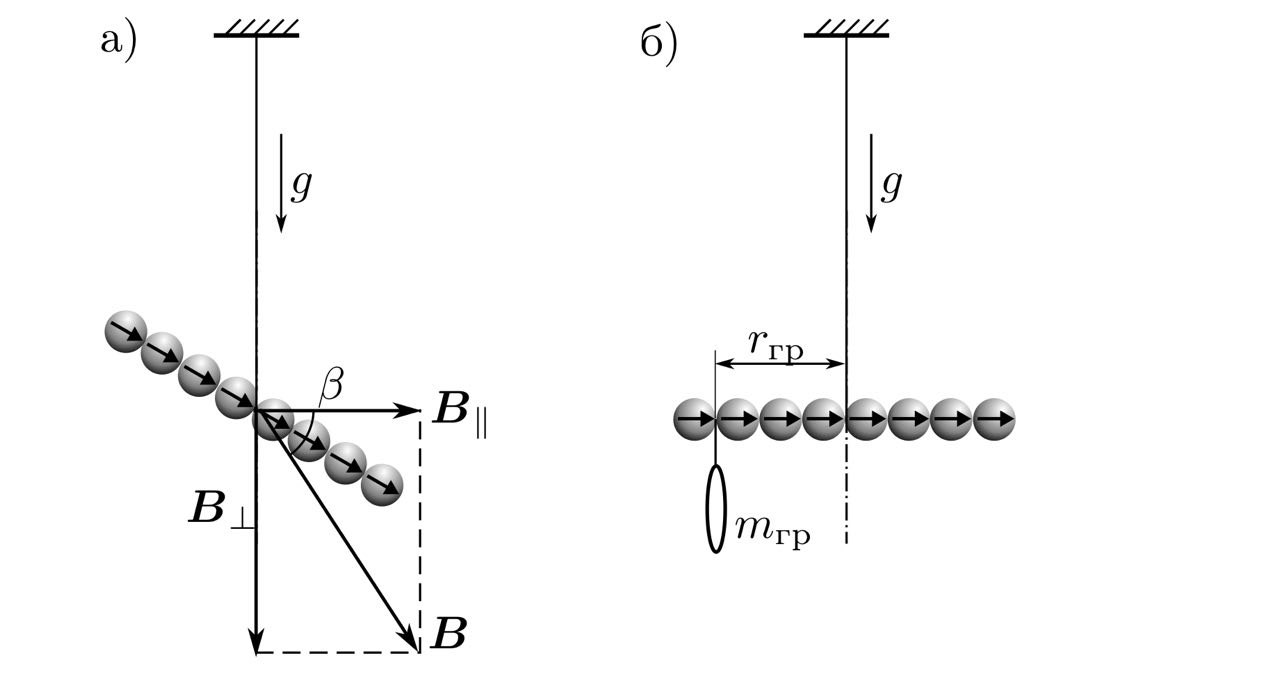
\includegraphics[scale=0.21]{vert}
		\caption{Измерение вертикальной составляющей поля и магнитного наклонения}
		\label{vert}
	\end{figure}
	
	\begin{table}[H]
		\centering
		\begin{tabular}{|c|c|c|c|}
			\hline $n_{\text{шар}}$ & $m_{\text{гр}}$, г & $r_{\text{гр}}$, см& $\mathcal{M}$, H $\cdot $ м $\cdot 10^{-5}$ \\ \hline 
			4 & 0,356 &  0,6 & 2,095 \\ \hline
			6 & 0,193 & 1,2 & 2,722 \\ \hline
			8 & 0,176 & 1,8 & 3,108 \\ \hline
			10 & 0,227 & 2,4 & 5,344 \\ \hline
			12 & 0,146 & 3 & 4,297 \\ \hline
		\end{tabular}
		\caption{Зависимость момента от количества шариков в <<магнитной стрелке>>}
	\end{table}
	
	По полученным данным был построен график. В нем не учитывается точка при $n = 10$, сильно выбивается из общей зависимости.
	
	\begin{figure}[H]
		\centering
		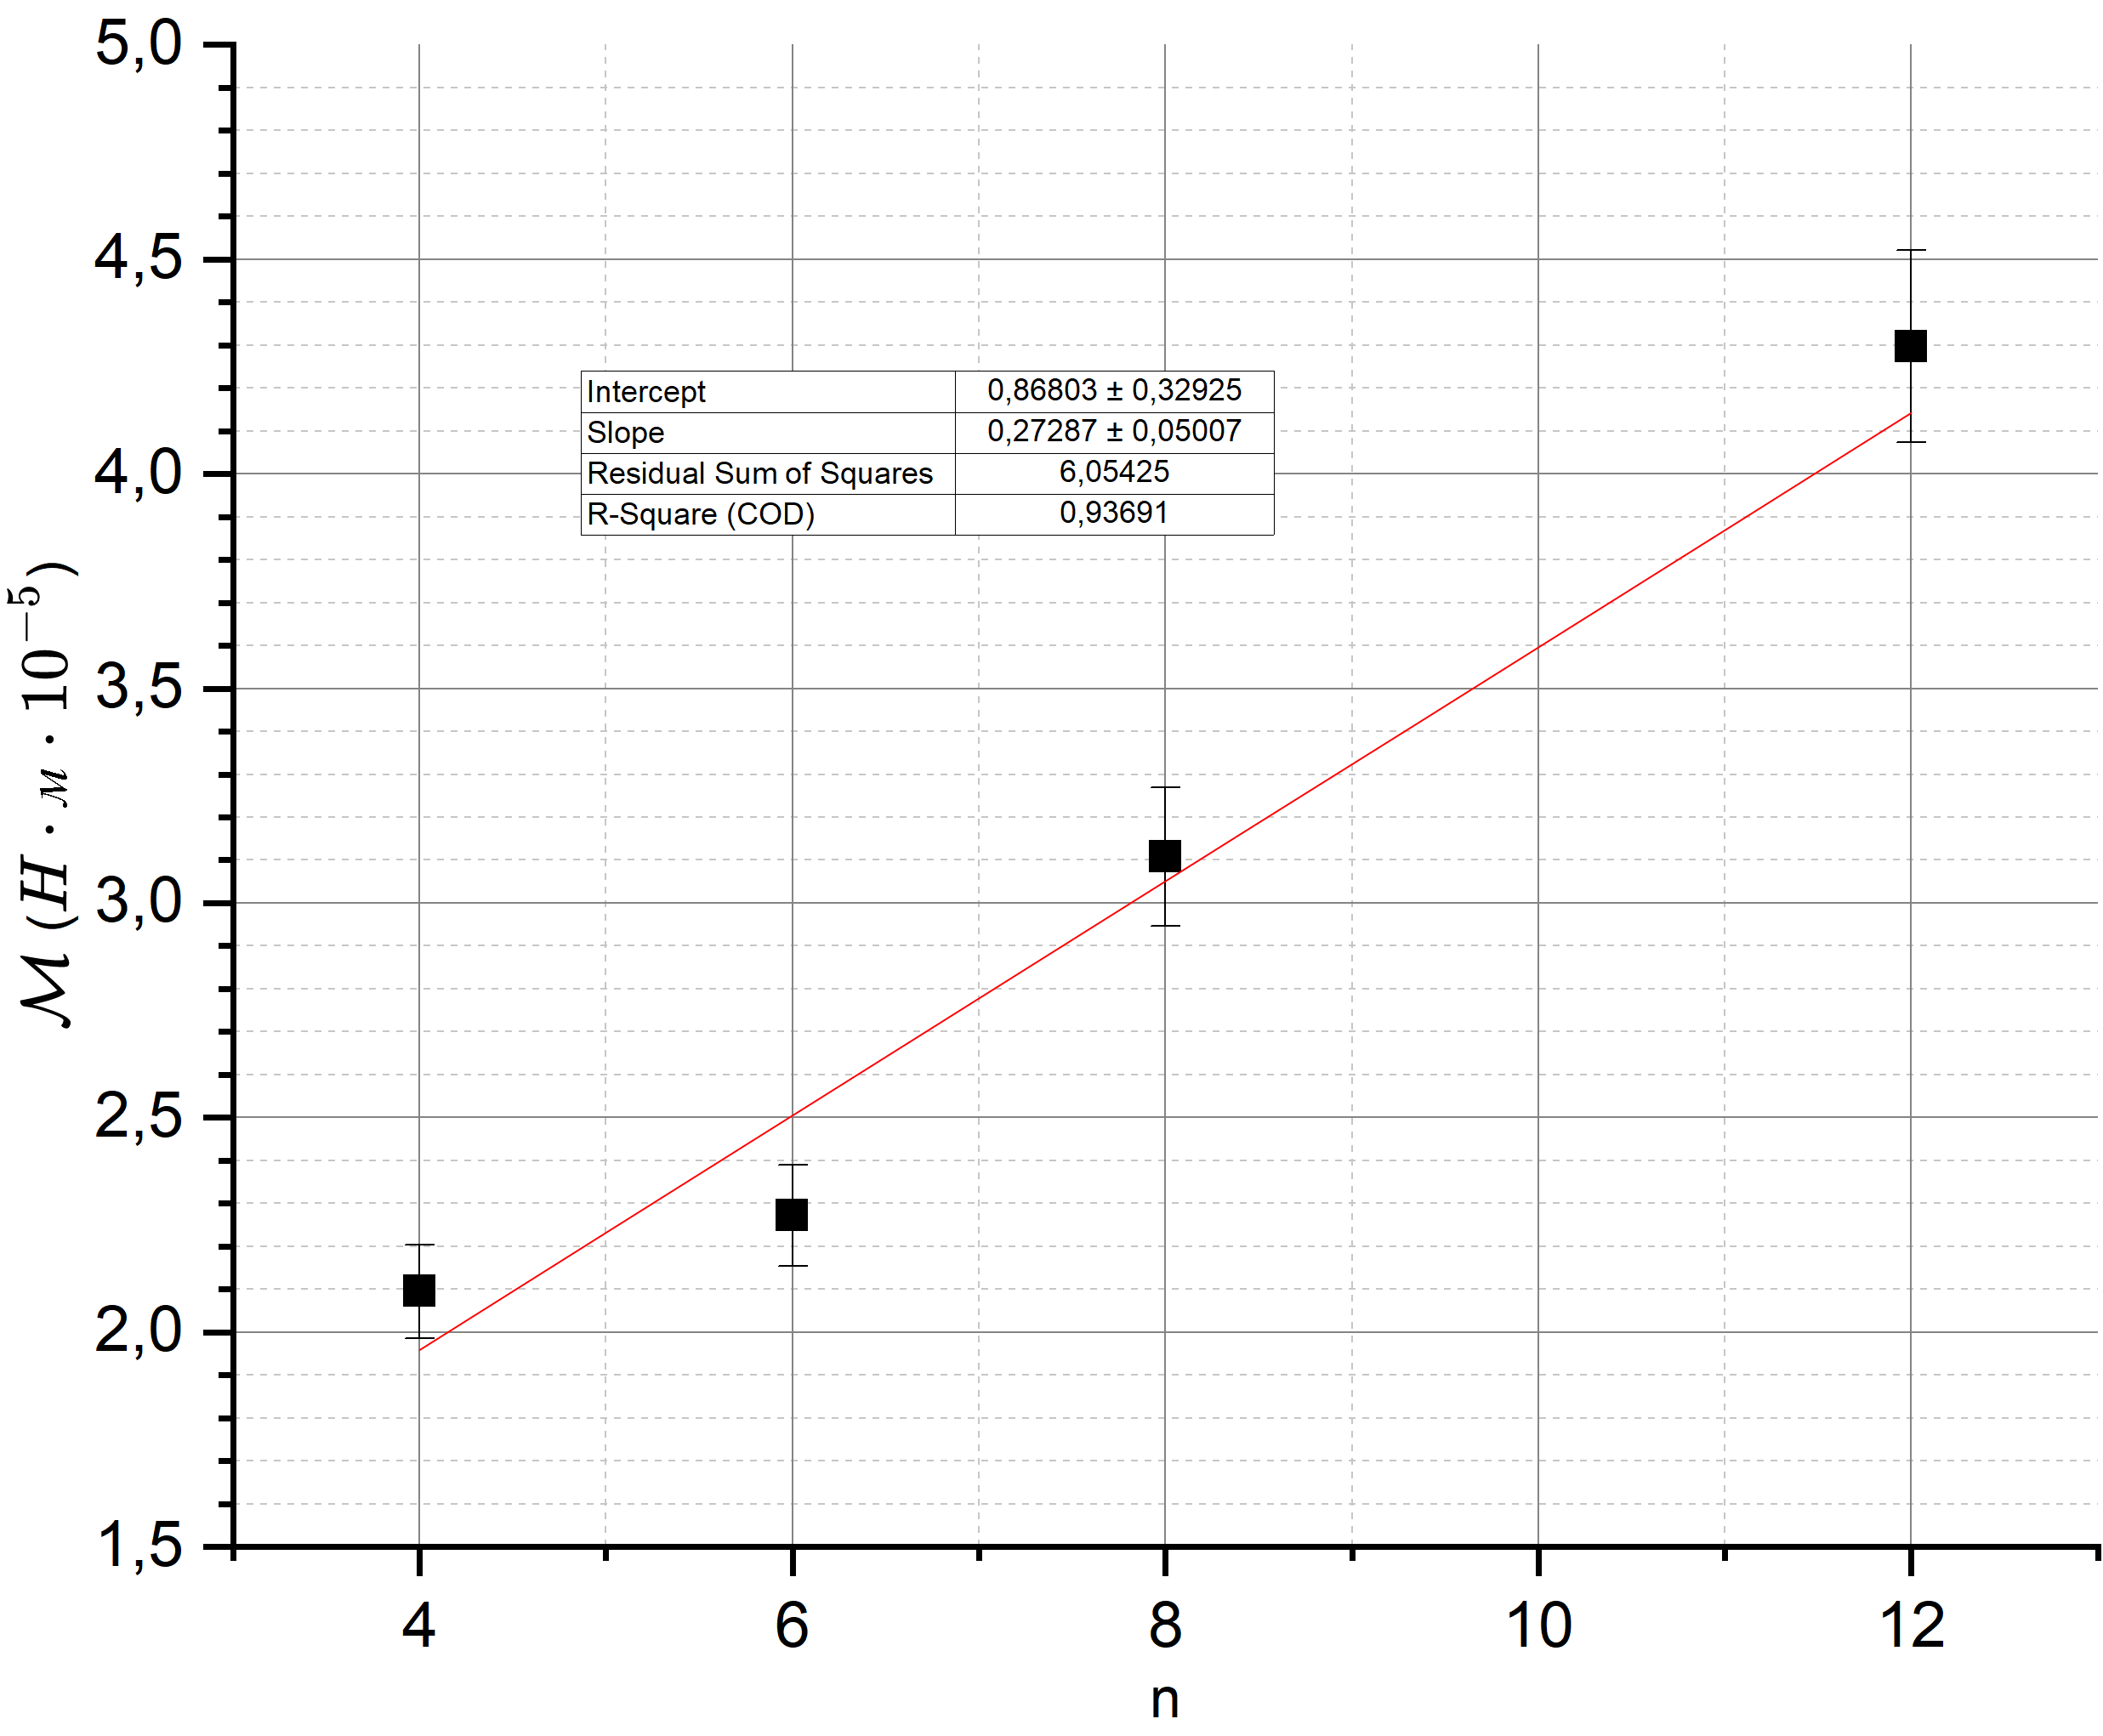
\includegraphics[width = \textwidth]{M(n)}
		\caption{График зависимости момента силы тяжести от количества шариков}
	\end{figure}
	
	Здесь принята погрешность измерения уравновешивающей массы за $5\%$. Выразим вертикальную составляющую магнитного поля:
	\[\mathcal{M}_n = m_{\text{гр}}gr_{\text{гр}} = n\mathbf{m}B_v\]
	\[B_v = \frac{\mathcal{M}_n}{n\mathbf{m}} = (3,72 \pm 0,69) \cdot 10^{-5} \ (\varepsilon = 18,6\%)\]
	
	Теперь можем посчитать полную величину индукции и магнитное наклонение:
	
	\[|B| = \sqrt{B_h^2 + B_v^2} = (4,38 \pm 0,66) \cdot 10^{-5} \ \ \text{Тл} \ (\varepsilon = 15\%) \]
	
	\[\tg{\beta} = \frac{B_v}{B_h} = 1,58 \pm 0,49 \ \ (\varepsilon = 31\%)\ \ \rightarrow \beta = 57,7^{\circ} \pm 8,9^{\circ} \ \ (\varepsilon = 15,5\%)\]
	
		Можно также рассчитать теоретическое значение $\beta$ на широте москвы $\varphi = 56^{\circ}$ в предположении, что Земля - однородно намагниченный шар:
	
	\[\beta = \arcctg{\frac{\frac{2P_m \sin{\varphi}}{R^3}}{\frac{-P_m \cos{\varphi}}{R^3}}} \approx -71^{\circ}\]
	
	Табличные данные магнитного поля в Москве приведены ниже:
	\[B_{\text{табл}} = 5 \cdot 10^{-5} \ \text{Тл} \ \ \ \beta_{\text{табл}} \approx 74^{\circ} - 78^{\circ}\]
	
	\section*{Выводы}
	В данной лабораторной работе были изучены характеристики неодимовых магнитов, а также вертикальная и горизонтальная составляющая магнитного поля. \\
	\begin{enumerate}
		\item Остаточная намагниченность $B_r = (0,814 \pm 0,047)$ Тл совпадает по порядку с табличными значениями $B_{r_{\text{табл}}} \approx 1,1$ Тл.
		\item Значения $B_h$ и $B_v$ также совпадают по порядку с табличными. По значению могут не совпадать, так как в кабинете еще есть электронные устройства, имеющие также своё магнитное поле. Полная величина индукции совпадает с табличными данными в пределах погрешности.
		\item Погрешности в измерениях компонент магнитного поля высоки ввиду неточности эксперимента, так как многое делается "на глаз".
		\item Магнитное наклонение не сходится с табличными данными. Скорее всего, причина, опять же, в наличии других источников полей в кабинете, ну и в неточности самого эксперимента.
	\end{enumerate}
	
	
\end{document}